\chapter{Organizzazione aziendale}
\begin{redbar}
Il concetto di \textbf{organizzazione}\index{Organizzazione aziendale} si riferisce alla struttura con cui si ordina un insieme di parti interdipendenti, ciascuna delle quali ha una funzione specifica e contribuisce al funzionamento dell’insieme complessivo.     
\end{redbar}

Questo sistema organizzato stabilisce centri decisionali, di controllo e operativi, definendo l’autorità e le responsabilità di ciascuno di essi. Gli elementi chiave dell’organizzazione includono l’organigramma, una rappresentazione visiva della struttura dell’azienda, le descrizioni delle mansioni e le procedure operative, che delineano come le funzioni debbano essere svolte.

\section{Struttura organizzativa}
Una \textit{struttura organizzativa}\index{Organizzazione aziendale!struttura organizzativa} può essere definita come l’insieme delle relazioni tra le persone che operano nell’impresa. Essa stabilisce come l’autorità e le responsabilità sono distribuite, e costituisce il fondamento dei processi operativi aziendali. Tuttavia, non deve essere considerata un modello astratto e ideale: ogni impresa deve adattare la propria struttura alla realtà concreta in cui si trova, tenendo conto delle persone, degli stili di gestione e dei meccanismi operativi già presenti.

In un’impresa, la struttura organizzativa comprende:
\begin{enumerate}
    \item \textit{Elementi hardware:} rappresentano la suddivisione delle funzioni aziendali in sub-unità specializzate;
    \item \textit{Elementi software:} comprendono norme, relazioni e obiettivi che regolano le attività dell’organizzazione.
\end{enumerate}

La struttura organizzativa può essere:
\begin{enumerate}
    \item \textit{Formale:} definisce chiaramente le divisioni di mansioni e i ruoli assegnati, spesso rappresentata tramite organigrammi che mostrano le relazioni gerarchiche tra le posizioni aziendali. 
    \item \textit{Informale:} si basa su rapporti spontanei e dinamiche di influenza non ufficiali, che possono incidere sul potere e sulle decisioni aziendali senza apparire nelle rappresentazioni formali.
\end{enumerate}

Gli \textit{organigrammi} forniscono una visione globale della struttura formale dell’impresa, evidenziando i principali ruoli e le relazioni tra le funzioni aziendali. Tuttavia, presentano alcuni limiti: non forniscono informazioni sull'importanza delle posizioni rappresentate, sui rapporti non gerarchici, né sull'ambiente di lavoro. Questi limiti vengono superati con documenti aggiuntivi, come i \textit{mansionari}, che descrivono i compiti assegnati a ciascuna posizione, e le \textit{norme procedurali}, che specificano come svolgere i singoli compiti.

\section{Evoluzione dei modelli organizzativi}
Per comprendere l’organizzazione aziendale attuale, è utile fare un passo indietro e considerare l’evoluzione dei modelli organizzativi.

\subsection*{Modello gerarchico}
Il \textit{modello gerarchico}\index{Organizzazione aziendale!Modello!gerarchico}, o struttura monofunzionale, rappresenta un’organizzazione rigida e centralizzata. In questo sistema, l’autorità e le competenze sono concentrate al vertice dell’impresa (\textit{principio di gerarchia}), mentre le funzioni vengono delegate verso il basso (\textit{principio di delega}). In caso di problemi o situazioni impreviste, le decisioni devono essere riportate ai vertici, i quali mantengono il controllo decisionale e forniscono indicazioni chiare (\textit{principio di eccezione}). Ogni persona nell’organizzazione deve sapere da chi ricevere ordini e a chi rivolgersi in caso di dubbi (\textit{principio dell'unità di direzione}).

\begin{figure}[ht]
    \centering
    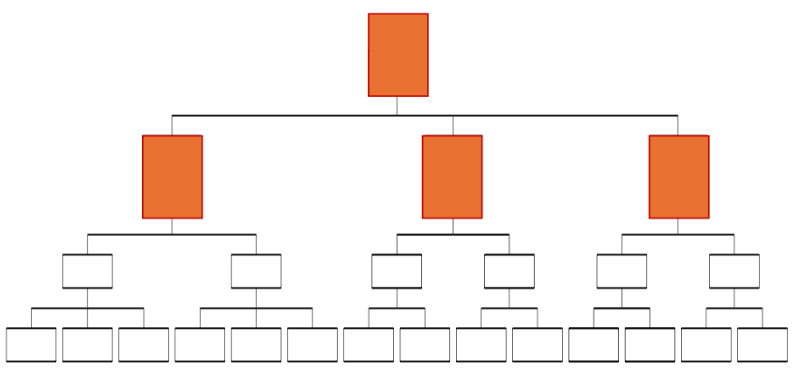
\includegraphics[width=0.6\linewidth]{images/modello-gerarchico.PNG}
    \caption{Modello gerarchico}
    \label{fig:modello-gerarchico}
\end{figure}

Il modello gerarchico è una struttura chiusa, efficace in un ambiente stabile, dove i cambiamenti del mercato avvengono lentamente rispetto alla capacità dell’impresa di adattarsi. Questa struttura facilita la comunicazione dall’alto verso il basso e consente un controllo totale da parte della direzione, che supervisiona tutte le funzioni aziendali.

\subsection*{Modello gerarchico-funzionale}
Un’evoluzione del modello gerarchico è la \textit{struttura gerarchico-funzionale}\index{Organizzazione aziendale!Modello!gerarchico-funzionale}, dove le attività aziendali vengono raggruppate per funzioni. Questo modello enfatizza la specializzazione, poiché ciascuna area funzionale, come marketing, produzione o contabilità, ha obiettivi specifici e competenze specializzate. In questa struttura, le decisioni strategiche rimangono centralizzate al vertice (\textit{principio di gerarchia}), mentre le funzioni sono organizzate in modo tale da favorire lo sviluppo di competenze e conoscenze specifiche (\textit{principio di conoscenza e specializzazione}).

\begin{figure}[ht]
    \centering
    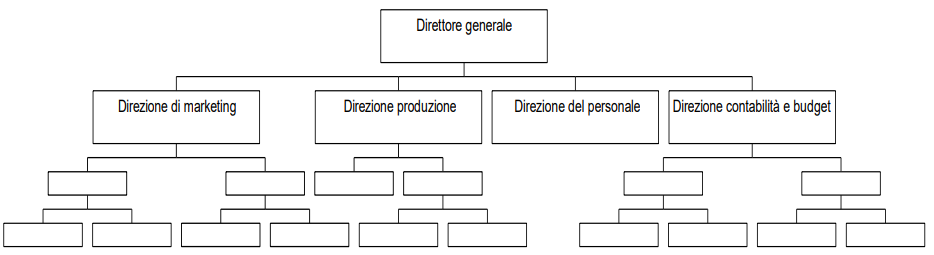
\includegraphics[width=0.8\linewidth]{images/modello-gerarchico-funzionale.PNG}
    \caption{Modello gerarchico-funzionale}
    \label{fig:modello-gerarchico-funzionale}
\end{figure}

Il modello gerarchico-funzionale è particolarmente utile quando l’efficienza e l’approfondimento delle competenze sono cruciali per il raggiungimento degli obiettivi aziendali. Tuttavia, presenta alcune limitazioni: la mancanza di coordinamento orizzontale tra le unità funzionali può rallentare la risposta dell’impresa ai cambiamenti esterni e limitare l’innovazione. Questo modello si adatta meglio ad aziende con un numero ristretto di prodotti, poiché facilita il coordinamento interno e consente di mantenere una visione chiara degli obiettivi funzionali.

Nel modello gerarchico-funzionale, l’organizzazione è suddivisa in tre livelli principali: 
\begin{enumerate}
    \item \textit{La direzione generale:} si occupa di amministrare l’azienda come un sistema unitario, definendo gli obiettivi primari e coordinando le varie aree funzionali. 
    \item \textit{I dipartimenti funzionali:} come marketing, produzione, personale e finanza, gestiscono le diverse funzioni aziendali, ma ciascuno si focalizza su obiettivi specifici legati alla propria area. 
    \item \textit{Le unità operative:} svolgono compiti esecutivi e implementano i piani dei dipartimenti, occupandosi di attività concrete come la produzione, la vendita o la ricerca.
\end{enumerate}
Nel modello gerarchico-funzionale, ciascun dipartimento ha funzioni specifiche che contribuiscono al funzionamento complessivo dell’impresa. 

\begin{enumerate}
    \item \textit{Direzione marketing.} La direzione marketing è responsabile della gestione del marketing mix, una combinazione di strumenti e strategie per raggiungere gli obiettivi di mercato dell'azienda. Questa direzione si occupa di:
    \begin{enumerate}
        \item \textit{Il prodotto e la sua filosofia:} il prodotto è considerato fondamentale per generare ricchezza, e deve rispondere ai bisogni dei consumatori e distinguersi dai concorrenti.
        \item \textit{Comunicazione:} include la pubblicità e le promozioni, ma anche l'incentivazione dei venditori.
        \item \textit{Distribuzione:} gestisce il trasferimento del prodotto dalla produzione al consumatore.
        \item \textit{Prezzo:} un elemento critico per la redditività aziendale, che deve riflettere il valore percepito e gli obiettivi economici.
    \end{enumerate}
    \item \textit{Direzione della produzione.} Questa direzione coordina il processo di trasformazione delle materie prime in prodotti finiti. Il responsabile della produzione si occupa della pianificazione dell'uso dei macchinari e della gestione dei ritmi produttivi, assicurando che le esigenze di mercato siano soddisfatte minimizzando i costi e ottimizzando le scorte.
    \item \textit{Direzione del personale.} Questa funzione si occupa della gestione delle risorse umane, dalla selezione all’assunzione del personale, e cura anche la retribuzione, i piani di carriera, le controversie sindacali e il rispetto delle norme di legge.
    \item \textit{Direzione amministrativa.} Si occupa della gestione contabile e fiscale dell'azienda, producendo report finanziari e rispettando gli obblighi legislativi in materia.
    \item \textit{Direzione finanziaria.} Responsabile della gestione del capitale, questa direzione si occupa di raccogliere e allocare risorse finanziarie, gestire i rapporti con le banche e supervisionare la gestione valutaria.
    \item \textit{Direzione ricerca e sviluppo (R\&S).} La direzione R\&S si focalizza sull'innovazione di prodotto e di processo, assicurando così la competitività e la sostenibilità futura dell'azienda.
\end{enumerate}

\begin{Example}{Caso di studio - Apple}{}
\textit{Un esempio di modello gerarchico-funzionale è Apple.} 

Apple è un’organizzazione con una struttura gerarchica che include un CEO al vertice. Sotto di lui troviamo varie direzioni, come Design, Hardware, Software e Marketing, ognuna con responsabilità specifiche ma che rispondono al vertice.

Apple ha evoluto la propria struttura organizzativa per adattarsi a differenti fasi di sviluppo, passando da un modello funzionale a un modello divisionale, e infine ritornando al funzionale, riflettendo così le strategie e le priorità aziendali nel tempo.    
\end{Example}

\subsection*{Modello divisionale}
Il \textit{modello divisionale}\index{Organizzazione aziendale!Modello!divisionale} organizza l'azienda attraverso divisioni separate, ciascuna delle quali è responsabile di prodotti, servizi o programmi specifici. Ogni divisione viene trattata come una piccola unità operativa autonoma il cui scopo principale è gestire e massimizzare i ricavi derivanti dal prodotto o dal servizio che rappresenta. Questa struttura si adatta a organizzazioni che producono diversi beni o servizi, consentendo a ciascuna divisione di concentrarsi su obiettivi specifici.

\begin{figure}[ht]
    \centering
    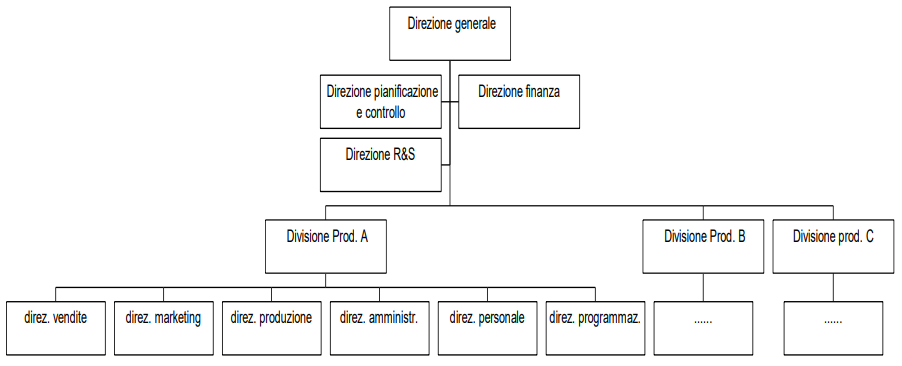
\includegraphics[width=0.8\linewidth]{images/modello-divisionale.PNG}
    \caption{Modello divisionale}
    \label{fig:modello-divisionale}
\end{figure}

Nel modello divisionale, il processo decisionale è decentralizzato, permettendo alle divisioni di operare con una maggiore autonomia rispetto alla struttura gerarchica. Inoltre, il coordinamento tra le unità funzionali è ottimizzato in base ai prodotti. Tuttavia, il modello presenta anche alcuni punti di debolezza: elimina le economie di scala, poiché ogni divisione gestisce le proprie operazioni in modo autonomo, e riduce la specializzazione tecnica poiché le divisioni tendono a operare in modo indipendente. Questo modello è particolarmente adatto ad ambienti caratterizzati da rapidi cambiamenti e a grandi organizzazioni con un'ampia varietà di prodotti o servizi.

\subsection*{Modello per area geografica}
Simile al modello divisionale, questa struttura\index{Organizzazione aziendale!Modello!area geografica} organizza l’azienda in divisioni geografiche, cioè separate per area di mercato (America, Europa, Asia, ecc.), in modo da adattarsi alle esigenze specifiche di ciascuna regione. Questo approccio permette una maggiore personalizzazione delle strategie aziendali e una migliore gestione delle risorse locali, facilitando l’espansione in nuovi mercati.

\begin{figure}[ht]
    \centering
    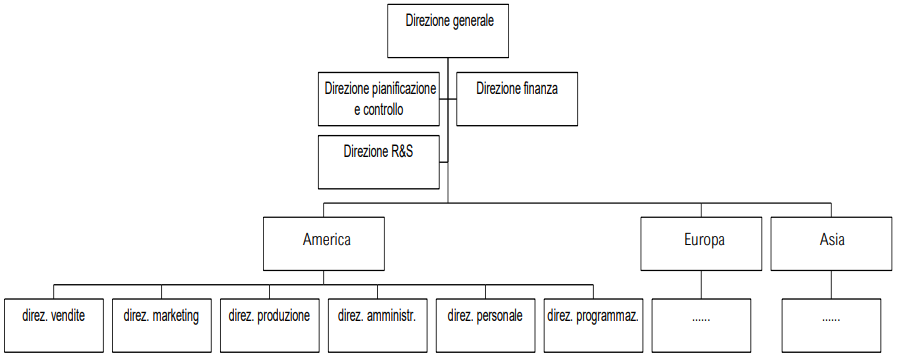
\includegraphics[width=0.8\linewidth]{images/modello-area-geografica.PNG}
    \caption{Modello per area geografica}
    \label{fig:modello-area-geografica}
\end{figure}

La struttura per area geografica consente all’azienda di espandersi in modo efficace nei mercati esteri, grazie a una gestione adattata alle necessità locali. Tuttavia, la decentralizzazione comporta costi amministrativi elevati e richiede un coordinamento accurato per mantenere un equilibrio tra le aree. Anche in questo modello, il processo decisionale è decentralizzato, il che facilita la risposta rapida alle esigenze di ogni mercato.

\subsection*{Modello a matrice}
La \textit{struttura a matrice}\index{Organizzazione aziendale!Modello!matrice} si distingue per la flessibilità e l’apertura dell’impresa verso un ambiente dinamico, combinando i vantaggi dell’organizzazione per funzioni (ad esempio marketing, finanza, produzione) con quelli dell’organizzazione per prodotti o progetti. In questo modello, ogni unità organizzativa può rispondere a due strutture di autorità: una basata sulla funzione aziendale e una orientata al progetto o al prodotto.

\begin{figure}[ht]
    \centering
    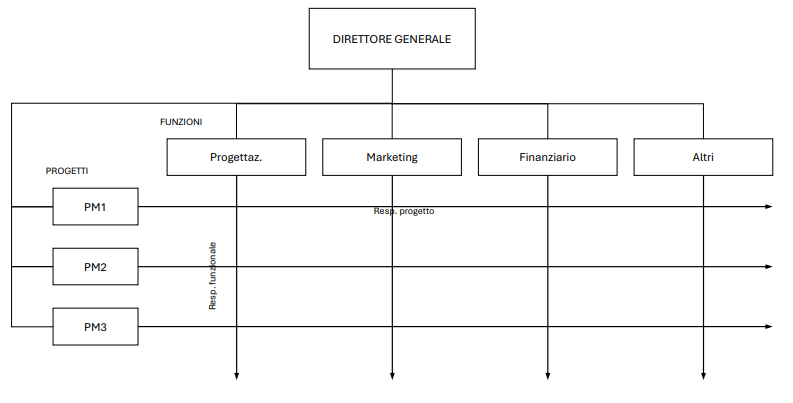
\includegraphics[width=0.8\linewidth]{images/modello-matrice.PNG}
    \caption{Modello a matrice}
    \label{fig:modello-matrice}
\end{figure}

Il modello a matrice è efficace in contesti dove è essenziale il coordinamento orizzontale e richiede sia un alto livello di competenze tecniche sia innovazione. Tuttavia, l’esposizione a una duplice autorità può generare confusione e richiede un buon livello di competenze interpersonali per gestire efficacemente le dinamiche di lavoro. Questo modello è indicato per aziende di media dimensione, con una varietà di prodotti, che devono affrontare contesti in rapido cambiamento.

\subsection*{Modello a rete e outsourcing}
La \textit{struttura a rete}\index{Organizzazione aziendale!Modello!rete e outsourcing} estende la collaborazione oltre i confini dell'azienda, affidando a partner esterni parte delle funzioni aziendali (outsourcing). L’azienda si concentra sul core business, mantenendo al proprio interno le attività che forniscono un vantaggio competitivo, mentre esternalizza le altre, come la produzione o la logistica.

\begin{figure}[ht]
    \centering
    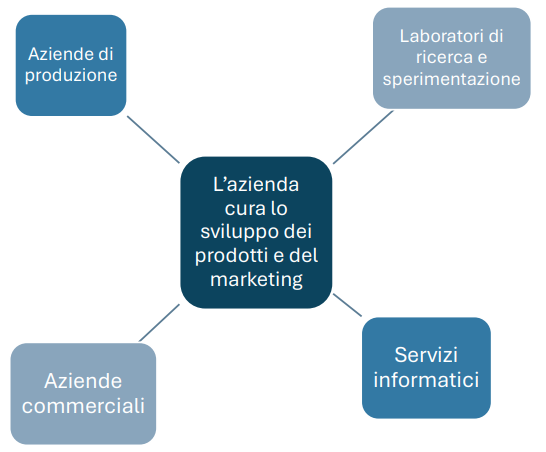
\includegraphics[width=0.5\linewidth]{images/modello-rete-outsourcing.PNG}
    \caption{Modello a rete e outsourcing}
    \label{fig:modello-rete-outsourcing}
\end{figure}

Questa struttura offre all'azienda una notevole flessibilità, riducendo i costi e permettendo di adattarsi rapidamente ai cambiamenti del mercato. D’altra parte, l’esternalizzazione può portare a un controllo limitato sulle attività delegate, con rischi legati alla continuità e alla qualità dei servizi forniti dai partner. Il modello a rete è particolarmente utile per aziende piccole e medie che necessitano di una presenza globale senza sostenere grandi investimenti infrastrutturali.